% !TEX TS-program = pdflatex
% !BIB program = bibtex
%
% IEEE T-RO Regular Paper — Double-Anonymous Submission Scaffold
% Generated: 2026-05-09 (P161 tro-template-conversion-scaffold)
% Status: skeleton — section structure, figure/table placeholders, and
%         citation keys. No fabricated results. Content must be filled
%         from paper/manuscript_en_thick.md.
% Compile: pdflatex main && bibtex main && pdflatex main && pdflatex main

\documentclass[journal]{IEEEtran}

% ── Packages ────────────────────────────────────────────────────────
\usepackage{graphicx}
\usepackage{amsmath,amssymb}
\usepackage{booktabs}
\usepackage{hyperref}
\usepackage{multirow}
\usepackage{cite}          % IEEE-style compressed numeric citations

% ── Double-anonymous settings ───────────────────────────────────────
% T-RO requires double-anonymous review. The initial submission must
% not include author names, affiliations, acknowledgments, or
% identifying funding disclosures.
\newcommand{\blind}{[BLINDED — ADD AFTER ACCEPTANCE]}

\begin{document}

\title{Dynamic Industrial Semantic-Segmentation-Assisted SLAM:\\
Object-Centric Map Maintenance via Open-Vocabulary\\
Object-Instance Filtering}

\author{\blind}
\thanks{\blind}

\maketitle

% ── Abstract ────────────────────────────────────────────────────────
\begin{abstract}
Dynamic industrial environments challenge semantic SLAM because stable
infrastructure, movable equipment, forklifts, carts, people, and temporary
cargo can appear in the same RGB-D observations. A semantic map that admits
every segmented object as persistent structure risks semantic drift and
dynamic-object contamination. This paper studies semantic-segmentation-assisted
SLAM for dynamic industrial environments as a principled session-level map
admission control problem. Starting from an RGB-D open-vocabulary frontend
based on Grounding DINO~\cite{liu2024grounding}, SAM2
segmentation~\cite{ravi2024sam2}, OpenCLIP reranking~\cite{cherti2023reproducible},
and 2D-to-3D object initialization, we build an object-centric maintenance
layer that converts segmentation-derived detections into
\emph{ObjectObservations}, session-level \emph{TrackletRecords},
cross-session \emph{MapObjects}, and revisioned map updates. The key mechanism
is explicit admission control rather than raw detection yield: persistence,
stability, and dynamicity signals determine whether segmented semantic evidence
is retained as stable landmark support or rejected as transient or dynamic
contamination. We evaluate the current system on TorWIC industrial RGB-D
revisits~\cite{barath2023povslam} under same-day, cross-day, and cross-month
Aisle protocols, with Hallway retained as a separate 10-session
broader-validation branch. The primary Aisle ladder reaches
203/11/5, 240/10/5, and 297/14/7 for frame-level objects, cross-session
clusters, and retained stable objects; the Hallway branch reaches 537/16/9
over 80/80 executed first-eight Hallway frames. The results support a bounded
systems claim: segmentation-assisted semantic observations can become auditable
long-term SLAM map evidence when filtered through cross-session stable-object
retention and dynamic-contamination rejection rules.
\end{abstract}

% ── Index Terms ─────────────────────────────────────────────────────
% Note: T-RO no longer requires IEEE keywords/index terms in many
% recent author guidelines. If required, uncomment and fill:
% \begin{IEEEkeywords}
% Semantic SLAM, dynamic SLAM, semantic segmentation, long-term mapping,
% open-vocabulary perception, object-level mapping, industrial robotics,
% RGB-D perception, map maintenance.
% \end{IEEEkeywords}

% ────────────────────────────────────────────────────────────────────
%  I. INTRODUCTION
% ────────────────────────────────────────────────────────────────────
\section{Introduction}
\label{sec:introduction}

\subsection{Motivation}
\label{sec:motivation}

Industrial mobile robots operate in environments that change repeatedly over
time. A warehouse aisle, assembly area, or logistics corridor may contain
persistent infrastructure, semi-static work equipment, and dynamic agents
within the same field of view. Long-term SLAM motivates map reuse across such
revisits~\cite{cadena2016past}, while dynamic SLAM shows why moving or
semi-static objects must be handled explicitly rather than treated as rigid
background structure~\cite{bescos2018dynaslam}. A semantic-segmentation-assisted
SLAM system must therefore answer a different question from a single-frame
segmenter or detector: which segmented semantic observations should become
persistent map evidence after repeated revisits, and which should be rejected
as dynamic or unreliable?

\subsection{The Admission-Control Gap}
\label{sec:admission-gap}

Open-vocabulary perception has made it practical to query arbitrary object
categories in real scenes~\cite{peng2023openscene,jatavallabhula2023conceptfusion}.
Object-level SLAM and open-vocabulary 3D mapping provide useful precedents for
compact landmarks and language-aligned 3D scene representations. However, these
outputs are not directly equivalent to durable map entities. Labels may drift,
masks may fragment across frames, dynamic agents may reappear in different
locations, and visually similar objects may be incorrectly merged. In
industrial settings, these errors are not minor: a persistent map polluted by
forklifts or temporary cargo can degrade later inspection, planning, or
navigation even when the original segmentation masks were visually plausible.

This work focuses on the maintenance layer between semantic segmentation,
open-vocabulary perception, and a long-term SLAM object map.

\subsection{Scope and Contribution Boundaries}
\label{sec:scope}

Instead of treating every segmentation-derived detection as a map update, we
explicitly represent frame-level observations, aggregate them within sessions,
associate them across sessions, and decide whether a cross-session object
should be retained as stable semantic landmark evidence. The goal is not to
claim a final lifelong SLAM backend, but to make the admission process
explicit, executable, and auditable on real industrial RGB-D data.

% TODO: fill Introduction body from manuscript_en_thick.md §I
% TODO: insert Fig.~1 (pipeline overview) here

\begin{figure}[t]
\centering
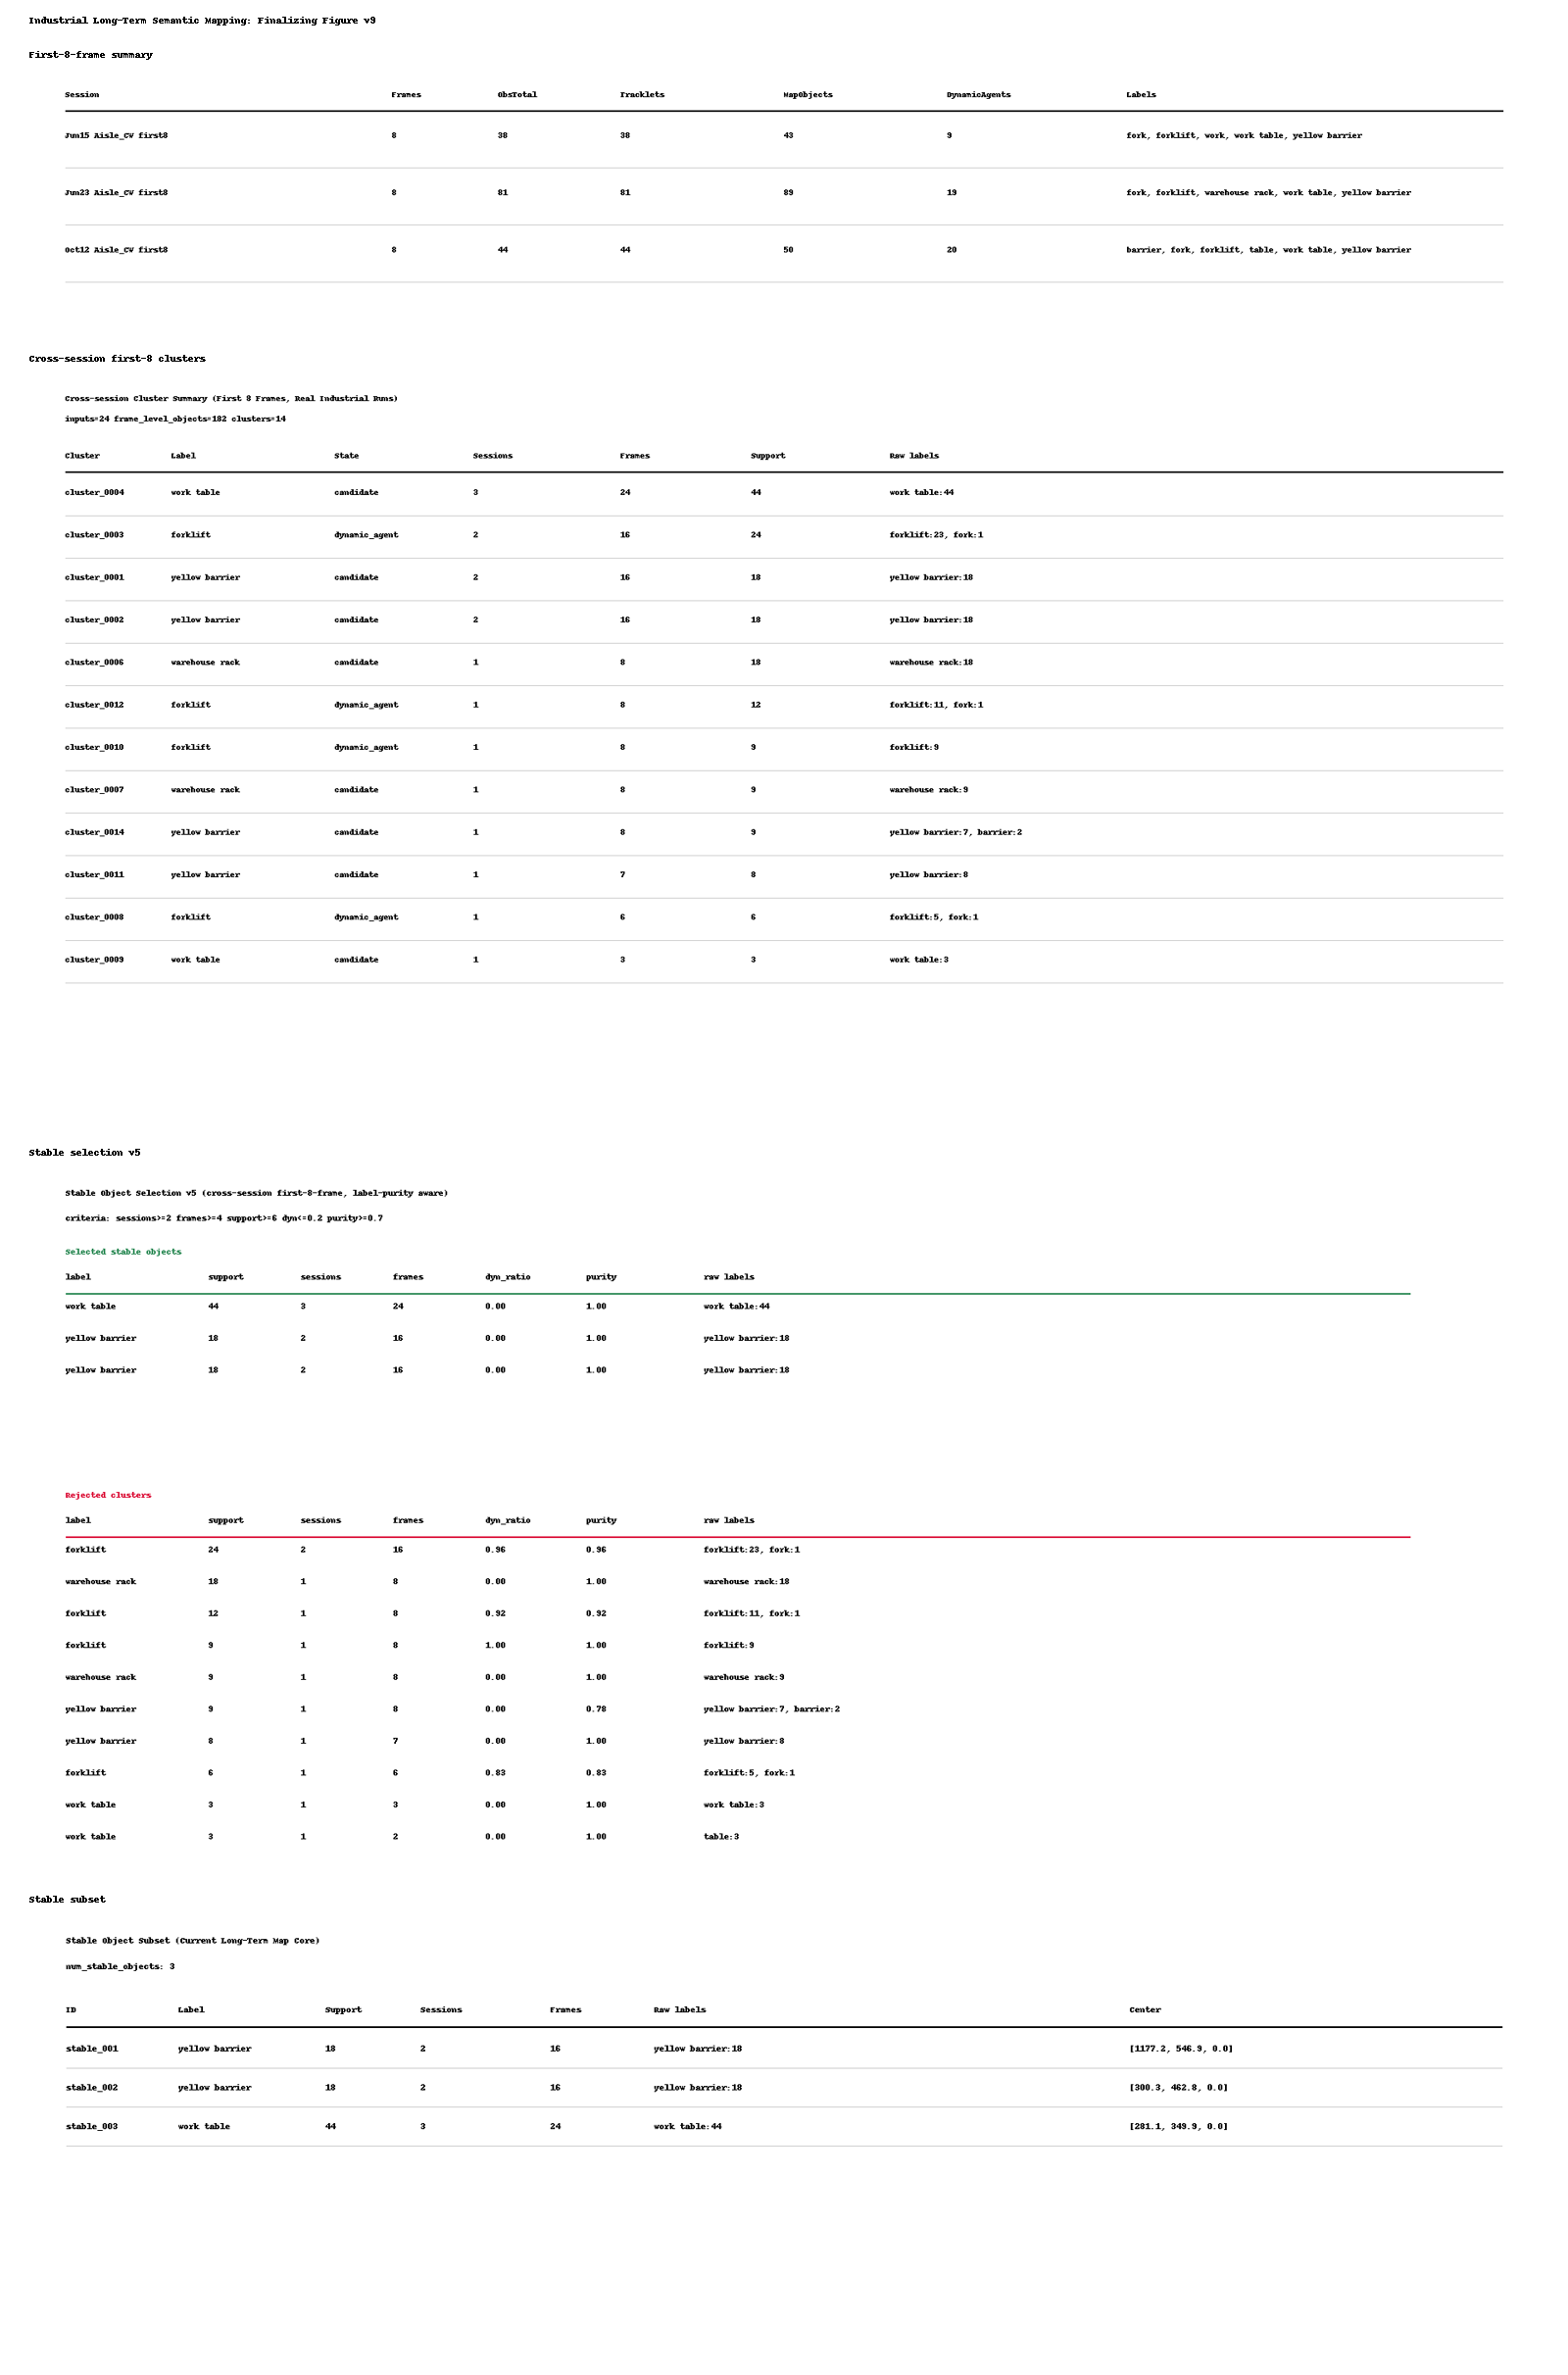
\includegraphics[width=\columnwidth]{../figures/torwic_paper_result_overview.png}
\caption{Semantic-segmentation-assisted SLAM maintenance pipeline.
Observation, tracklet, map-object, and revision layers.
\label{fig:pipeline}}
\end{figure}

% ────────────────────────────────────────────────────────────────────
%  II. CONTRIBUTIONS
% ────────────────────────────────────────────────────────────────────
\section{Contributions}
\label{sec:contributions}

% TODO: fill from manuscript_en_thick.md §II (8 items)

\begin{enumerate}
\item We formulate semantic-segmentation-assisted SLAM in dynamic industrial
  environments as a principled session-level map-admission control problem over
  segmented semantic observations, repeated revisits, and dynamic-object
  contamination.
\item We implement an object-centric maintenance pipeline that converts
  open-vocabulary RGB-D segmentation outputs into ObjectObservations,
  TrackletRecords, MapObjects, and MapRevisions.
\item We introduce interpretable persistence, stability, and dynamicity
  signals that decide whether semantic evidence is retained as stable landmark
  support or rejected as transient/dynamic evidence.
\item We define a TorWIC multi-session evaluation protocol spanning same-day,
  cross-day, cross-month, and Hallway broader-validation revisit settings
  without promoting secondary Hallway evidence into the primary Aisle ladder.
\item We provide current evidence showing stable-object retention,
  dynamic-contamination rejection, and map-admission selectivity on real
  industrial RGB-D data.
\item \textbf{[TODO: fill items 5--8 from manuscript\_en\_thick.md §II]}
\end{enumerate}

% ────────────────────────────────────────────────────────────────────
%  III. RELATED WORK
% ────────────────────────────────────────────────────────────────────
\section{Related Work}
\label{sec:related-work}

\subsection{Semantic SLAM and Object-Level Mapping}
\label{sec:semantic-slam}

% TODO: fill from manuscript_en_thick.md §III.A

\subsection{Dynamic SLAM and Dynamic-Object Suppression}
\label{sec:dynamic-slam}

% TODO: fill from manuscript_en_thick.md §III.B

\subsection{Long-Term Map Maintenance and Stable Landmark Reuse}
\label{sec:map-maintenance}

% TODO: fill from manuscript_en_thick.md §III.C

\subsection{Segmentation-Assisted Filtering and Open-Vocabulary 3D Mapping}
\label{sec:segmentation-filtering}

% TODO: fill from manuscript_en_thick.md §III.D

% ────────────────────────────────────────────────────────────────────
%  IV. PROBLEM FORMULATION
% ────────────────────────────────────────────────────────────────────
\section{Problem Formulation}
\label{sec:problem}

\subsection{Formal Statement}
\label{sec:formal}

% TODO: fill from manuscript_en_thick.md §IV.A

\subsection{Key Distinction from Standard SLAM}
\label{sec:distinction}

% TODO: fill from manuscript_en_thick.md §IV.B

% ────────────────────────────────────────────────────────────────────
%  V. METHOD
% ────────────────────────────────────────────────────────────────────
\section{Method}
\label{sec:method}

\subsection{Open-Vocabulary Object Observation Extraction}
\label{sec:observation-extraction}

% TODO: fill from manuscript_en_thick.md §V.A

\subsection{Session-Level Tracklet Records}
\label{sec:tracklets}

% TODO: fill from manuscript_en_thick.md §V.B

\subsection{Cross-Session MapObjects}
\label{sec:mapobjects}

% TODO: fill from manuscript_en_thick.md §V.C

\subsection{Stability and Dynamicity Scoring}
\label{sec:scoring}

% TODO: fill from manuscript_en_thick.md §V.D

The trust score for an object $O$ is defined as:
\begin{equation}
\tau(O) = S_{\text{persist}}(O) \cdot S_{\text{stable}}(O)
          \cdot (1 - S_{\text{dynamic}}(O))
\label{eq:trust}
\end{equation}

\subsection{Map Admission Criteria}
\label{sec:admission-criteria}

% TODO: fill from manuscript_en_thick.md §V.E

\subsection{Revisioned Map Updates}
\label{sec:revisions}

% TODO: fill from manuscript_en_thick.md §V.F

% ────────────────────────────────────────────────────────────────────
%  VI. EXPERIMENTAL PROTOCOL
% ────────────────────────────────────────────────────────────────────
\section{Experimental Protocol}
\label{sec:protocol}

\subsection{Dataset and Provenance}
\label{sec:dataset}

% TODO: fill from manuscript_en_thick.md §VI.A

\subsection{Protocol Design}
\label{sec:protocol-design}

% TODO: fill from manuscript_en_thick.md §VI.B

\subsection{Selection Criteria}
\label{sec:criteria}

% TODO: fill from manuscript_en_thick.md §VI.C

% ────────────────────────────────────────────────────────────────────
%  VII. RESULTS
% ────────────────────────────────────────────────────────────────────
\section{Results}
\label{sec:results}

\subsection{Primary Aisle Ladder}
\label{sec:aisle-results}

\begin{figure*}[t]
\centering
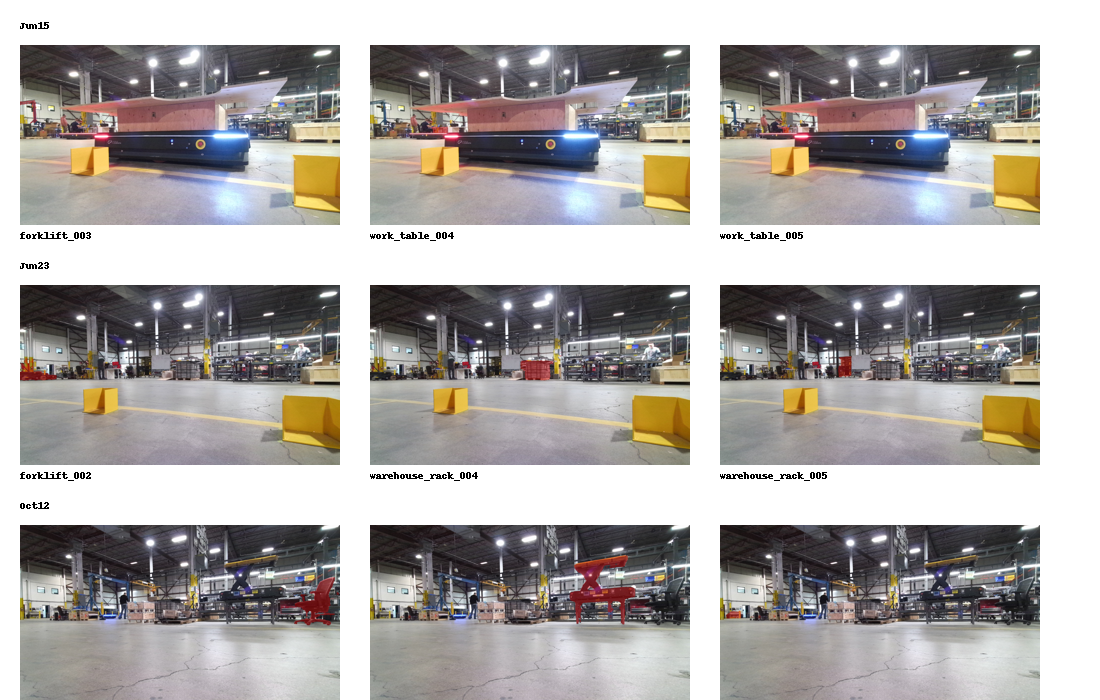
\includegraphics[width=\textwidth]{../figures/torwic_real_session_overlays.png}
\caption{Primary Aisle evidence ladder: same-day (203/11/5), cross-day
(240/10/5), cross-month (297/14/7). Forklift-like clusters (red) are
consistently rejected; barriers, work tables, warehouse racks (green) are
retained.
\label{fig:aisle-ladder}}
\end{figure*}

% TODO: fill text from manuscript_en_thick.md §VII.A

\begin{table}[t]
\centering
\caption{Primary Aisle Evidence Ladder}
\label{tab:aisle}
\begin{tabular}{lcccc}
\toprule
Setting & Sessions & Frame-Level & Clusters & Retained \\
\midrule
Same-day Aisle    &  4 & 203 & 11 & 5 \\
Cross-day Aisle   &  4 & 240 & 10 & 5 \\
Cross-month Aisle &  6 & 297 & 14 & 7 \\
\bottomrule
\end{tabular}
\end{table}

\subsection{Stable-Subset Composition}
\label{sec:stable-subset}

% TODO: fill from manuscript_en_thick.md §VII.B

\subsection{Hallway Broader-Validation}
\label{sec:hallway}

\begin{figure*}[t]
\centering
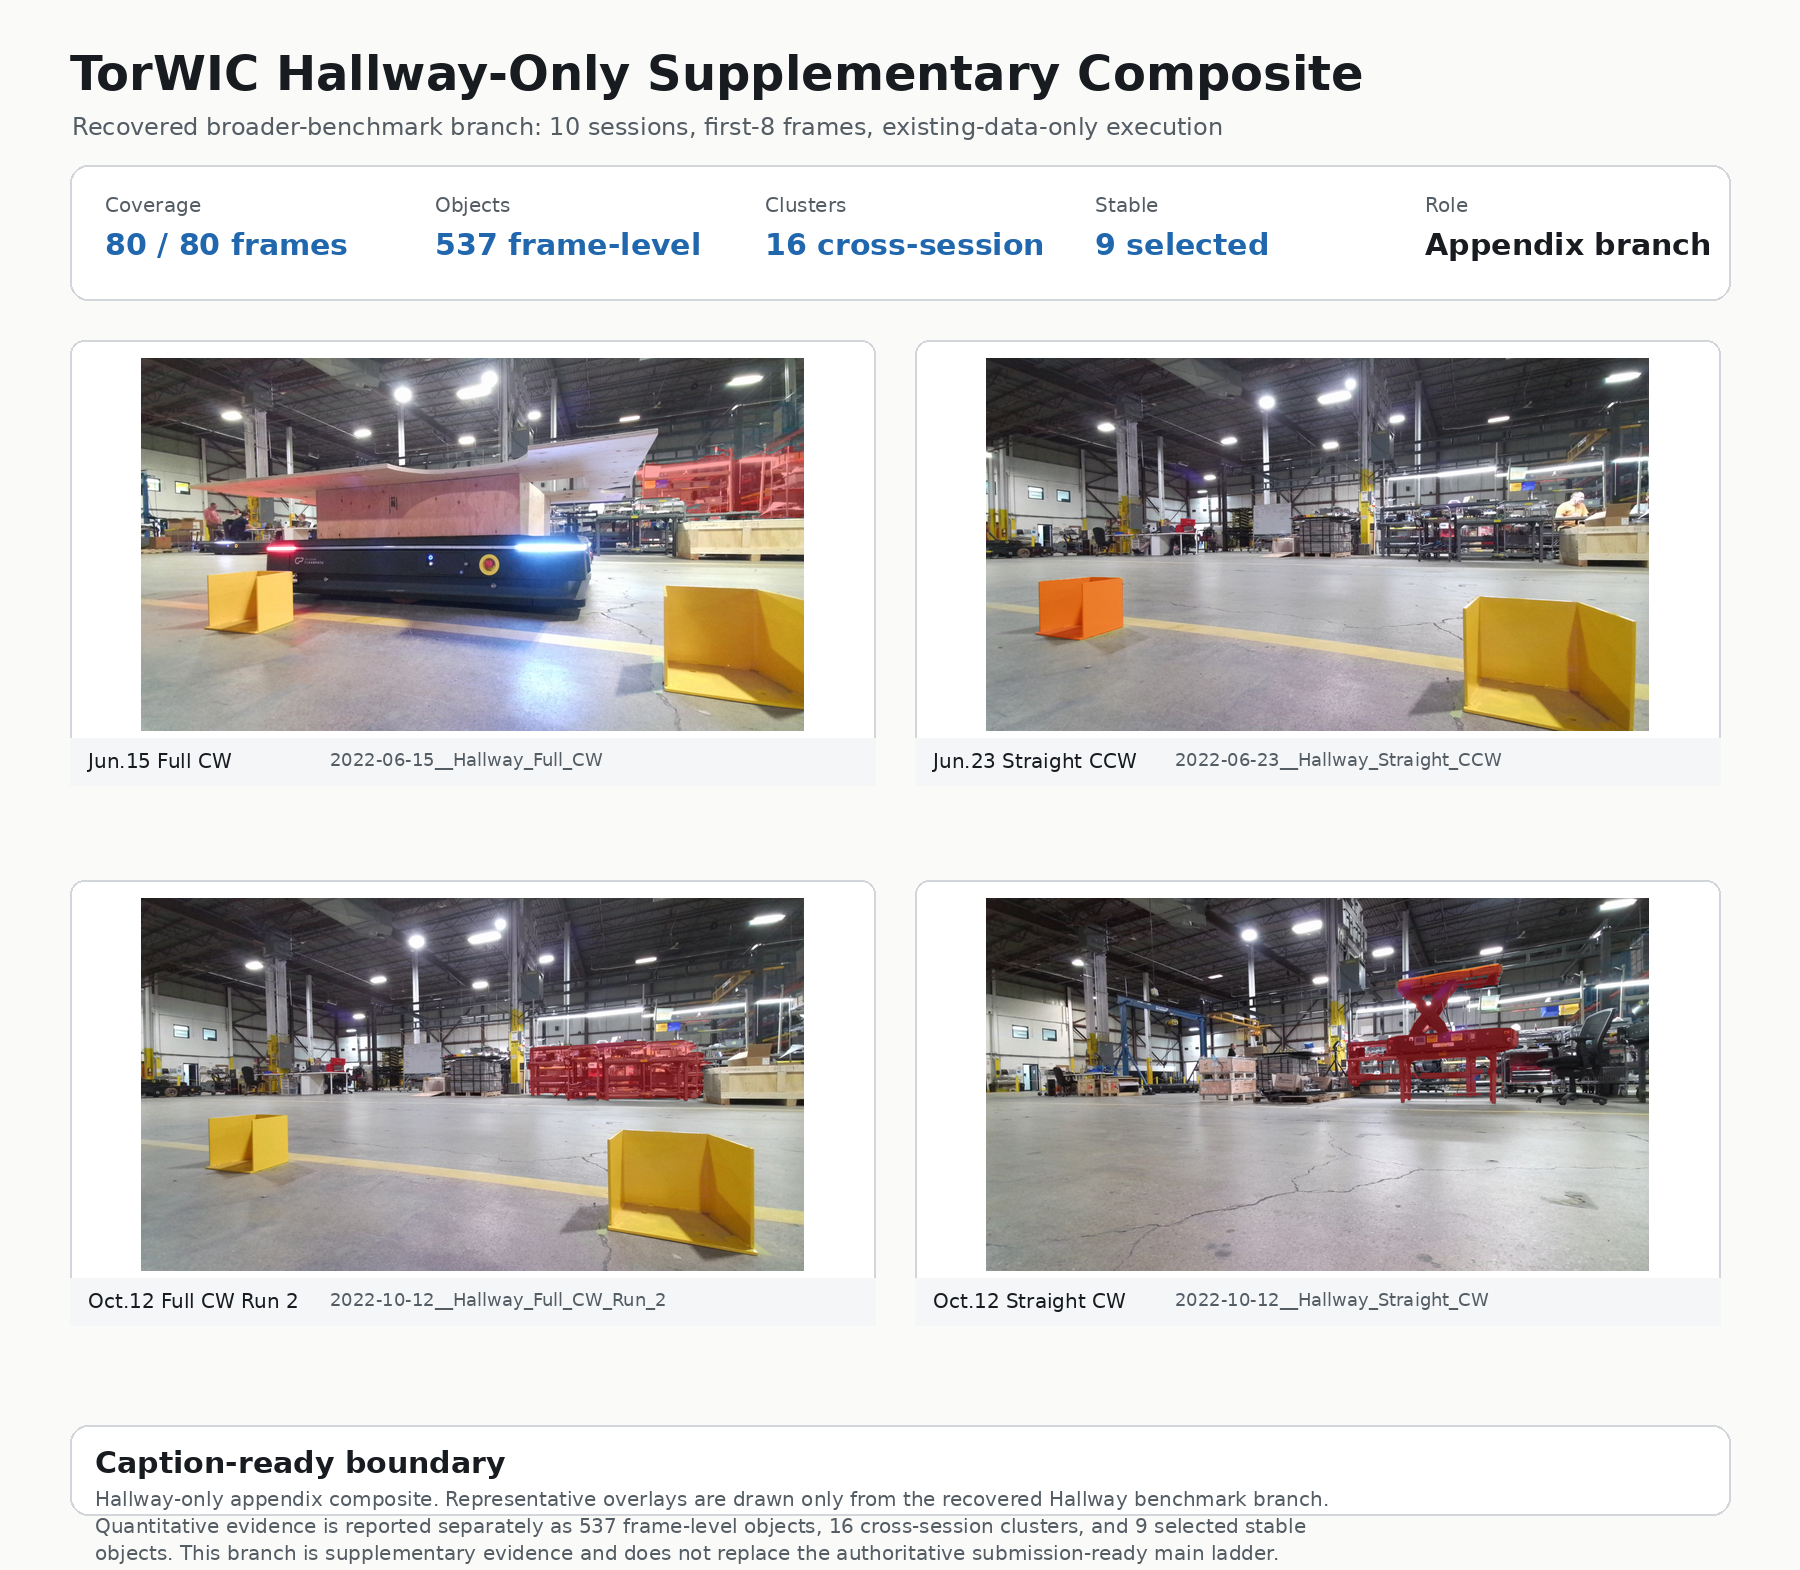
\includegraphics[width=\textwidth]{../figures/torwic_hallway_composite.png}
\caption{Hallway broader-validation composite (10 sessions, 537 frame-level
objects, 16 cross-session clusters, 9 retained stable objects). This branch
remains secondary and must not be merged into the primary Aisle ladder.
\label{fig:hallway}}
\end{figure*}

% TODO: fill from manuscript_en_thick.md §VII.C

\subsection{Dynamic-Contamination Rejection}
\label{sec:rejection}

% TODO: fill from manuscript_en_thick.md §VII.D

\begin{figure}[t]
\centering
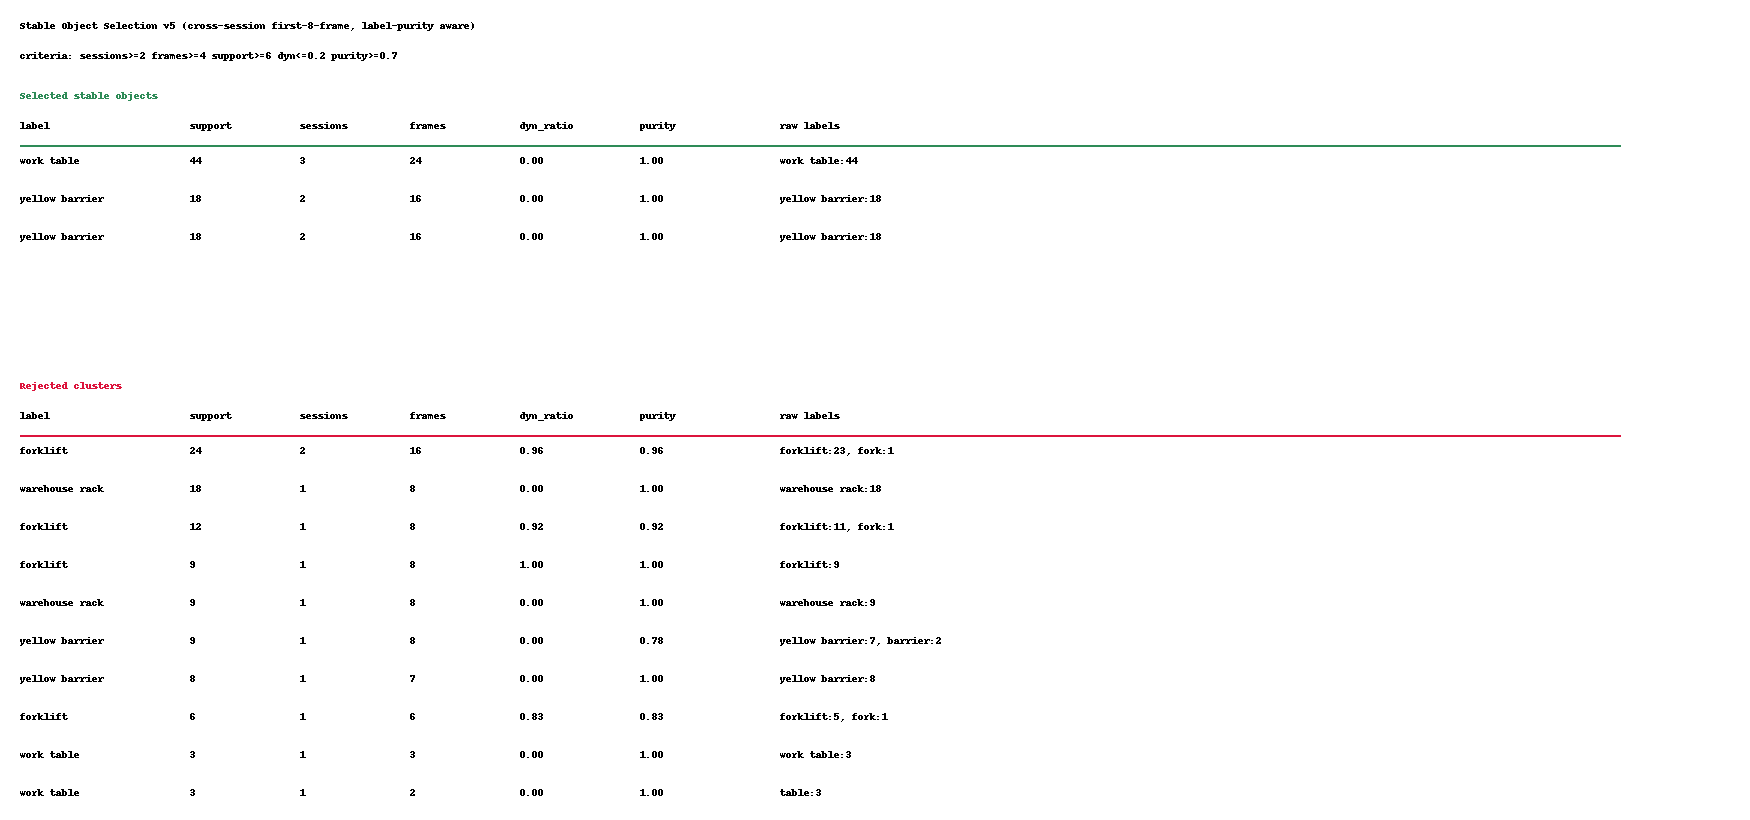
\includegraphics[width=\columnwidth]{../figures/torwic_stable_object_selection_v5.png}
\caption{Map-admission selectivity across all four protocols. Retained objects
(green) vs. rejected clusters (red, colored by rejection reason).
\label{fig:selectivity}}
\end{figure}

\subsection{Dynamic SLAM Backend Evaluation}
\label{sec:dynamic-backend}

% TODO: fill from manuscript_en_thick.md §VII.E

\begin{figure}[t]
\centering
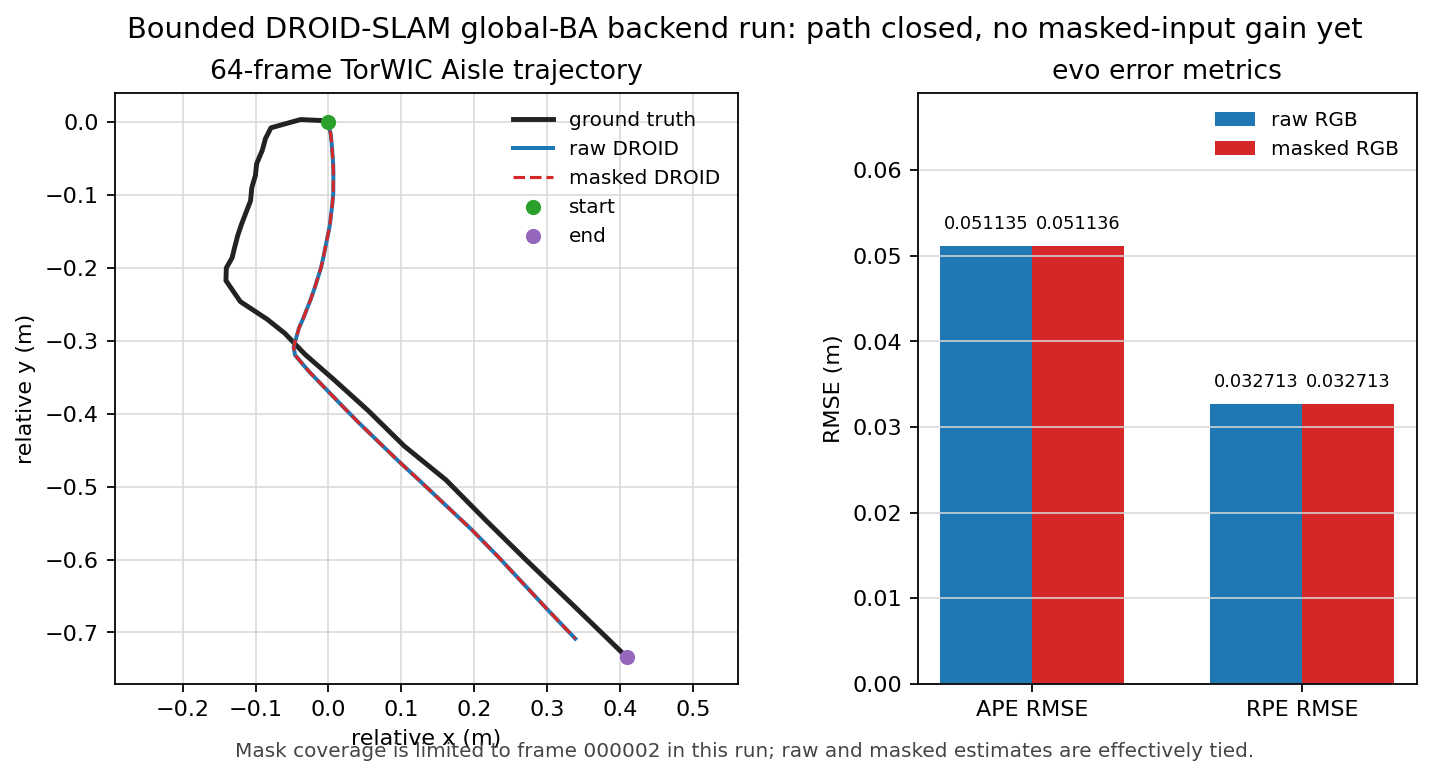
\includegraphics[width=\columnwidth]{../figures/torwic_dynamic_slam_backend_p134.png}
\caption{Bounded DROID-SLAM 64-frame global-BA raw-vs-masked backend
result~\cite{teed2021droidslam}. All 10 tested configurations produced
$|\Delta\text{ATE}| < 0.1$\,mm.
\label{fig:backend}}
\end{figure}

\subsection{Dynamic Masking Limitations}
\label{sec:masking-limits}

% TODO: fill from manuscript_en_thick.md §VII.F

\begin{figure}[t]
\centering
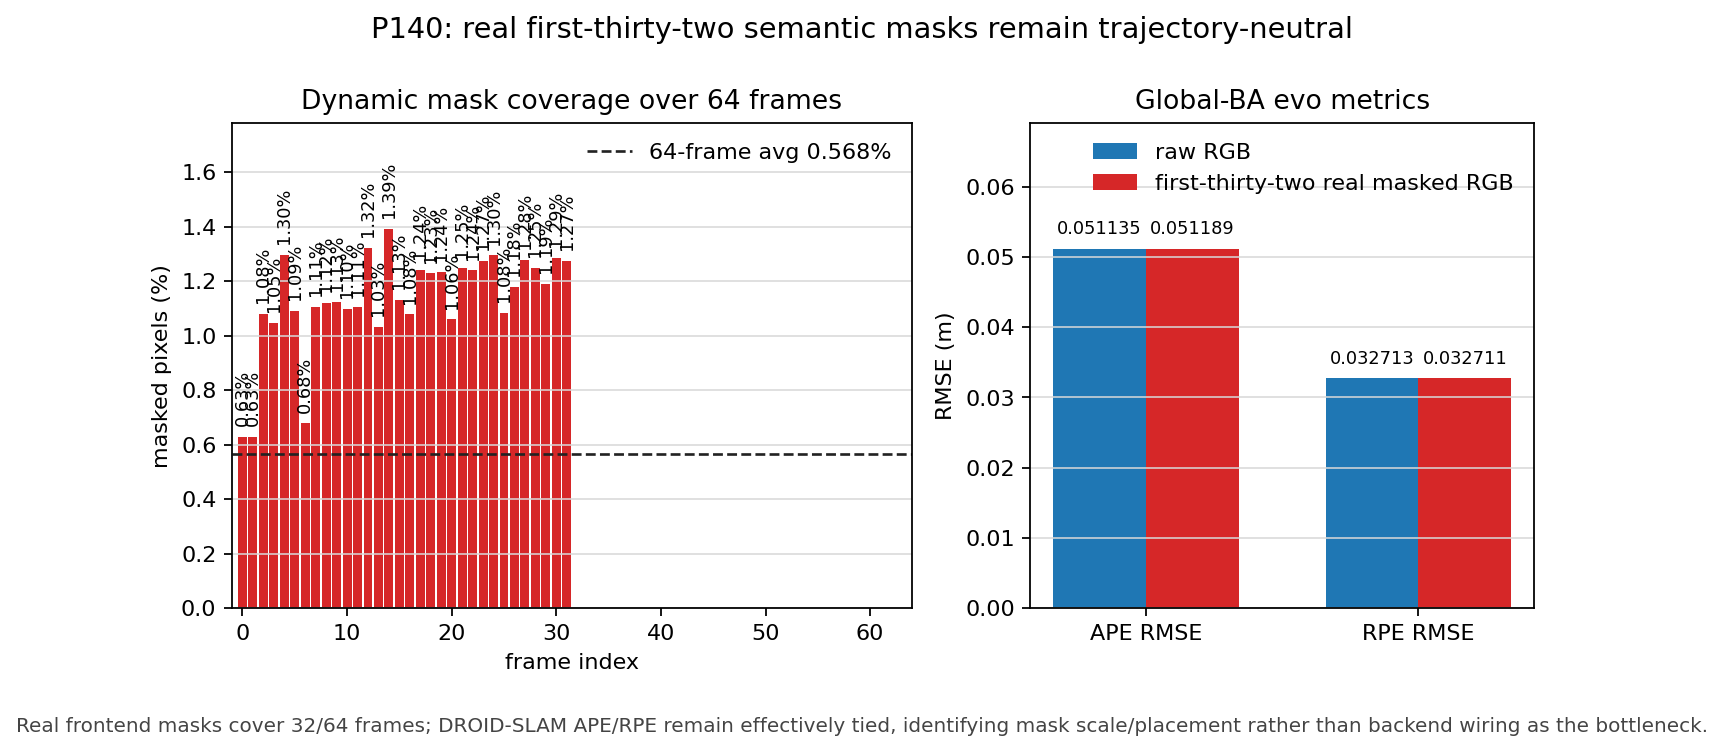
\includegraphics[width=\columnwidth]{../figures/torwic_dynamic_mask_first32_real_p140.png}
\caption{First-32 real semantic-mask backend diagnostic (strongest
configuration: 32/64 frames, 0.568\% mean mask coverage). ATE/RPE remain
effectively tied with raw RGB ($|\Delta\text{ATE}| < 0.1$\,mm).
\label{fig:mask32}}
\end{figure}

\subsection{Admission Criteria Defense}
\label{sec:admission-defense}

% TODO: fill from manuscript_en_thick.md §VII.G (P154-P157)

\subsubsection{Parameter Ablation (P154)}
\label{sec:ablation}

% TODO: fill from manuscript_en_thick.md §VII.G.1

\subsubsection{Baseline Comparison (P155)}
\label{sec:baseline}

% TODO: fill from manuscript_en_thick.md §VII.G.2

\begin{figure*}[t]
\centering
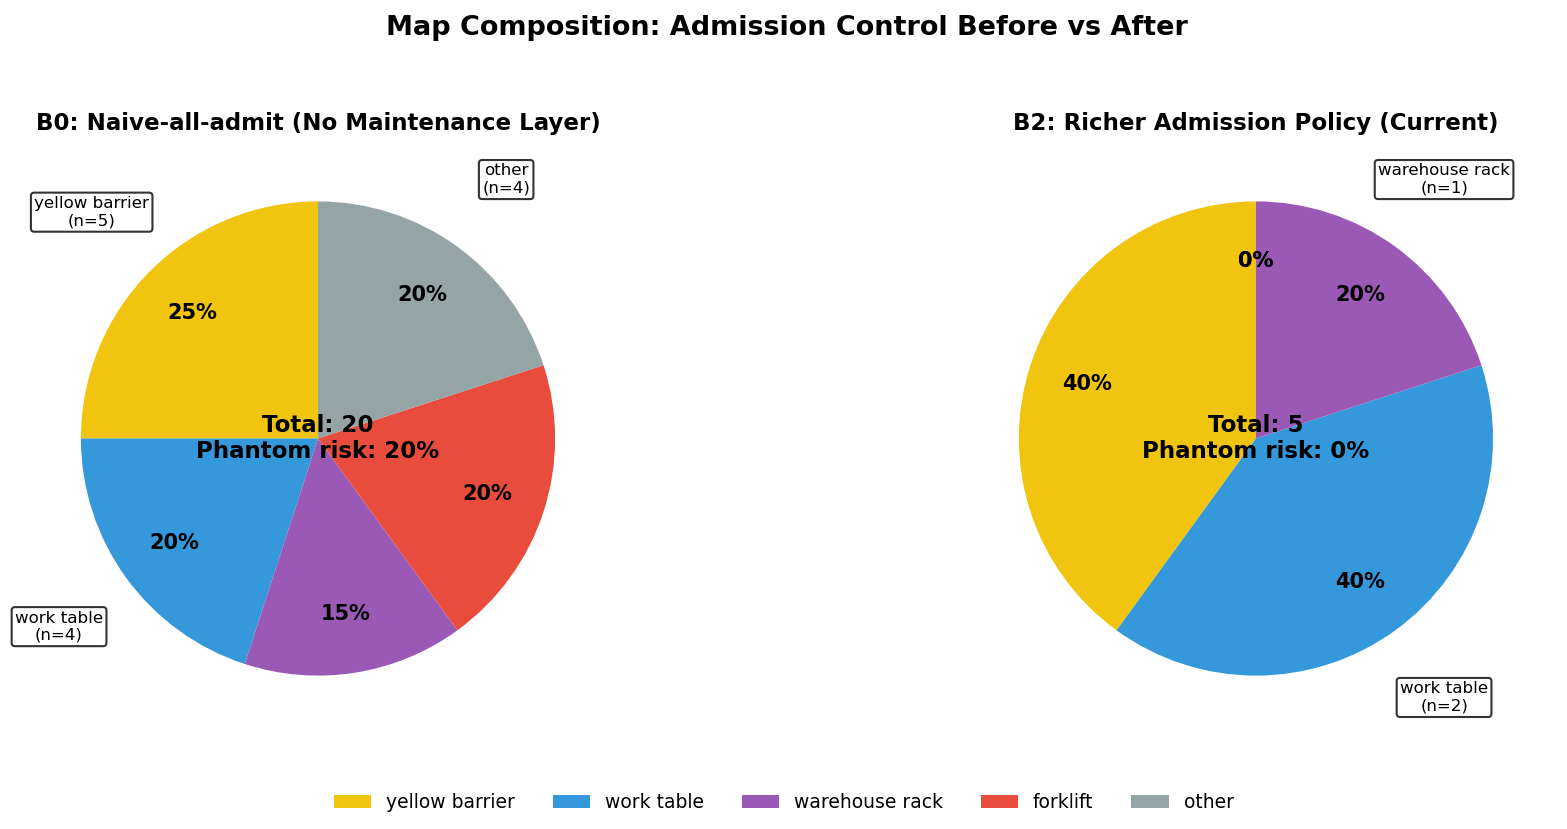
\includegraphics[width=\textwidth]{../figures/torwic_before_after_map_composition_p156.png}
\caption{Before/after map composition: B0 naive-all-admit (20 clusters,
4 forklifts = 20\% phantom risk) vs. B2 richer admission policy (5 verified
infrastructure, 0 forklifts).
\label{fig:composition}}
\end{figure*}

\begin{figure*}[t]
\centering
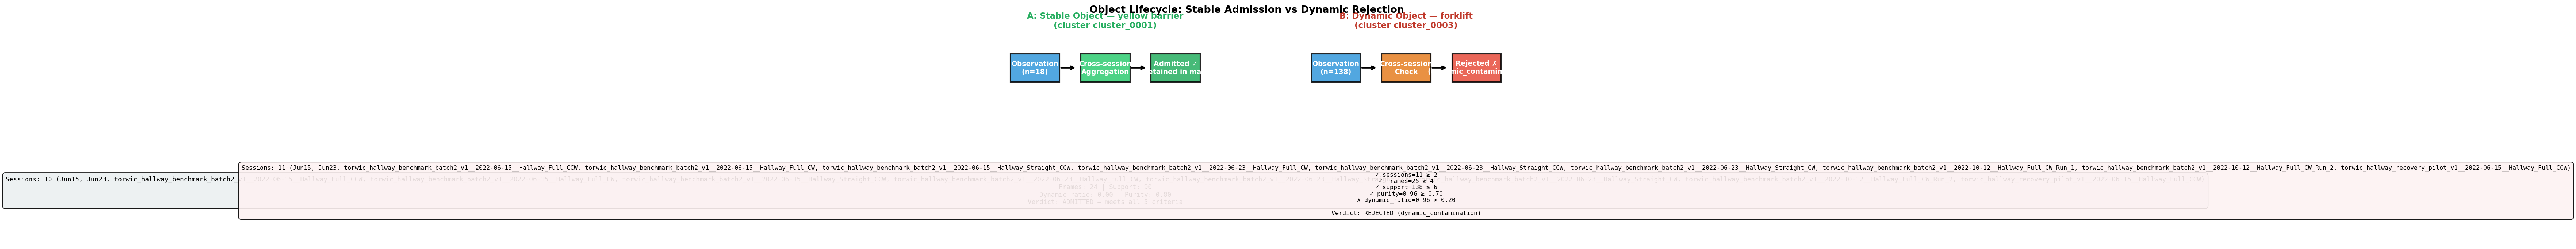
\includegraphics[width=\textwidth]{../figures/torwic_object_lifecycle_p156.png}
\caption{Object lifecycle: stable barrier (admitted — satisfies all 5
criteria) vs. forklift (rejected — dynamic\_contamination despite high purity
and support).
\label{fig:lifecycle}}
\end{figure*}

\begin{figure*}[t]
\centering
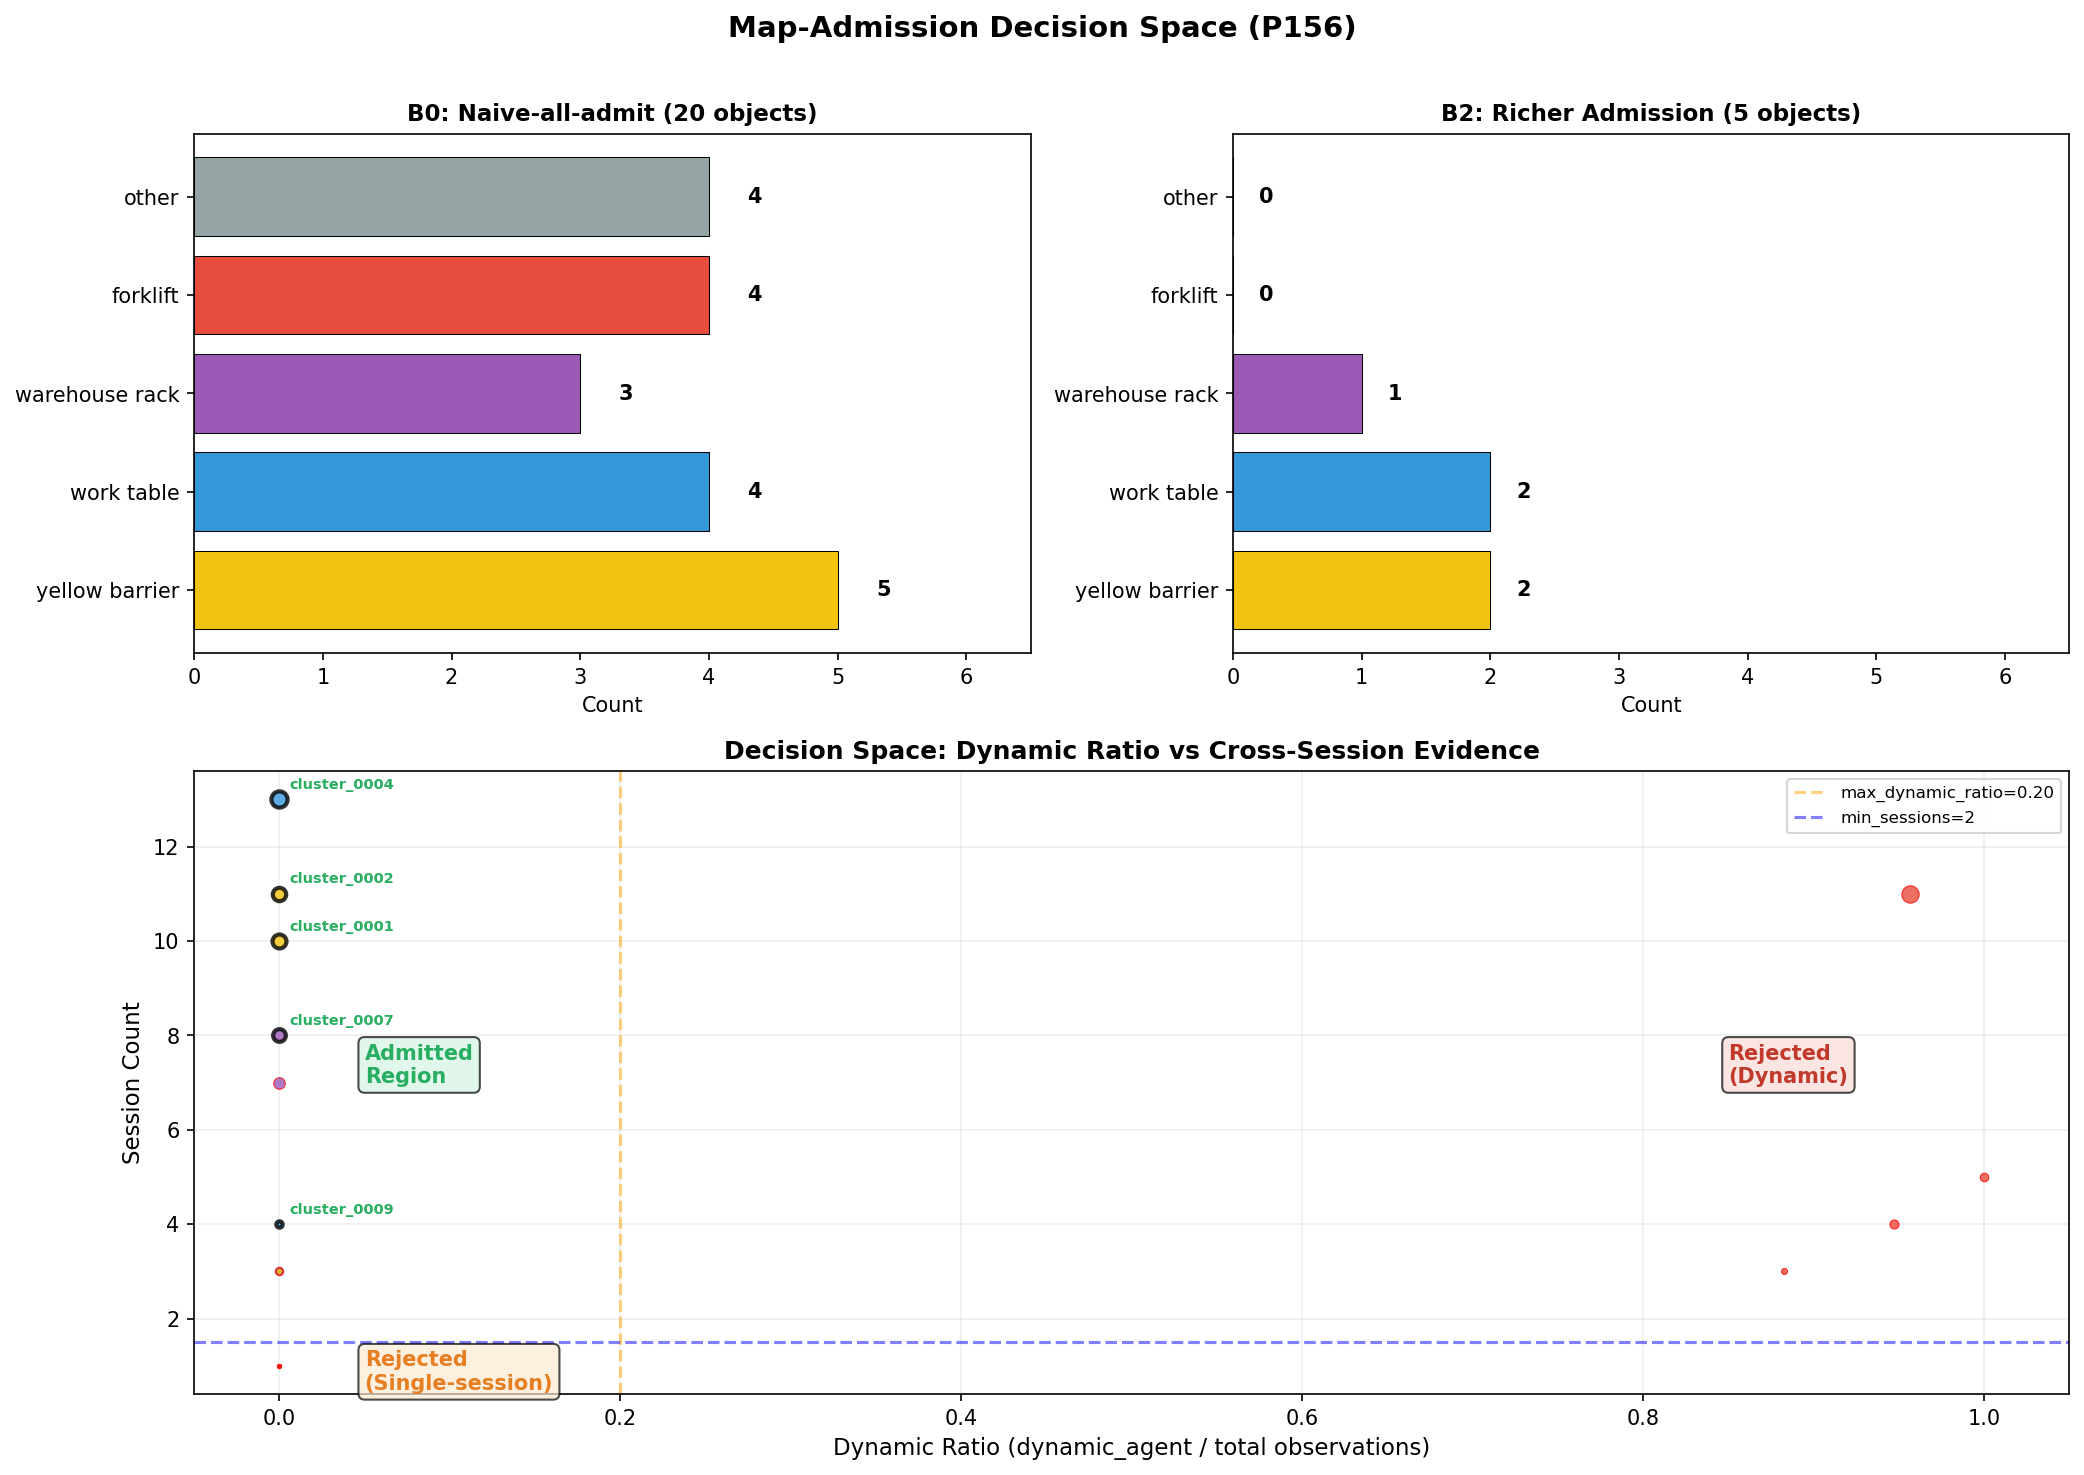
\includegraphics[width=\textwidth]{../figures/torwic_admission_decision_space_p156.png}
\caption{Admission decision space: dynamic\_ratio vs. session\_count for all
20 combined Aisle+Hallway clusters. Infrastructure clusters at ratio=0.00,
sessions $\geq$ 2; forklift clusters at ratio $\geq$ 0.83; zero clusters in
the intermediate range.
\label{fig:decision-space}}
\end{figure*}

\subsubsection{Per-Category Retention/Rejection Analysis (P157)}
\label{sec:category-analysis}

% TODO: fill from manuscript_en_thick.md §VII.G.3

\begin{figure}[t]
\centering
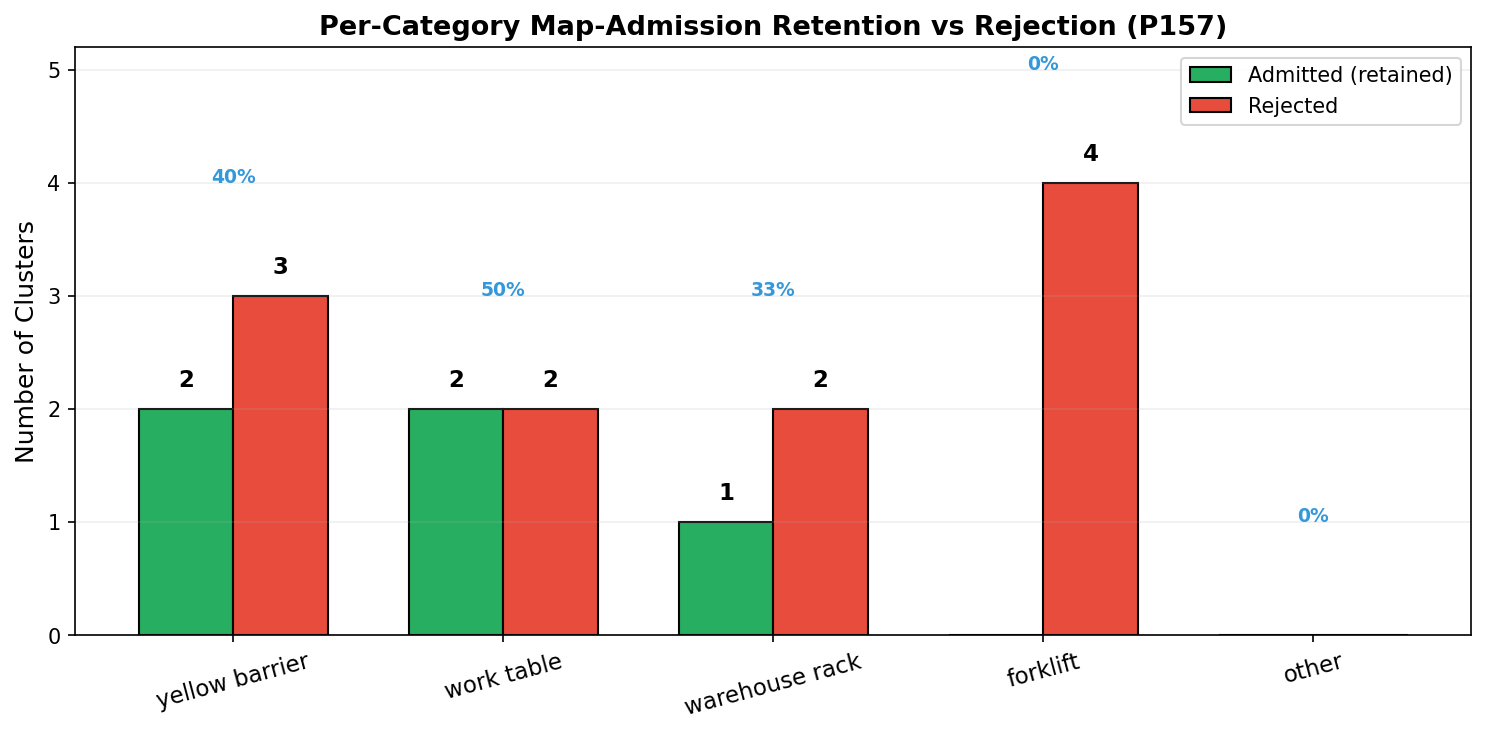
\includegraphics[width=\columnwidth]{../figures/torwic_per_category_retention_p157.png}
\caption{Per-category retention/rejection bar chart. Infrastructure retention:
33\%--50\%; forklift retention: 0/4 (0\%).
\label{fig:category-retention}}
\end{figure}

% ────────────────────────────────────────────────────────────────────
%  VIII. DISCUSSION
% ────────────────────────────────────────────────────────────────────
\section{Discussion}
\label{sec:discussion}

\subsection{Why Not Just Filter by Detection Confidence?}
\label{sec:disc-confidence}

% TODO: fill from manuscript_en_thick.md §VIII.A

\subsection{The Role of Session Count}
\label{sec:disc-sessions}

% TODO: fill from manuscript_en_thick.md §VIII.B

\subsection{Lightweight vs. Heavyweight}
\label{sec:disc-lightweight}

% TODO: fill from manuscript_en_thick.md §VIII.C

\subsection{Aisle vs. Hallway — Separate Roles}
\label{sec:disc-aisle-hallway}

% TODO: fill from manuscript_en_thick.md §VIII.D

% ────────────────────────────────────────────────────────────────────
%  IX. LIMITATIONS
% ────────────────────────────────────────────────────────────────────
\section{Limitations}
\label{sec:limitations}

% TODO: fill from manuscript_en_thick.md §IX (7 items)

\begin{enumerate}
\item Not a complete lifelong SLAM backend.
\item Larger-window or full-trajectory Hallway evaluation remains future work.
\item Rule-based association is not a final answer to long-term object identity.
\item No downstream task evaluation.
\item Venue-specific reference formatting is intentionally deferred.
\item Back-end model citations are provided~\cite{liu2024grounding,ravi2024sam2,cherti2023reproducible}.
\end{enumerate}

% ────────────────────────────────────────────────────────────────────
%  X. CONCLUSION
% ────────────────────────────────────────────────────────────────────
\section{Conclusion}
\label{sec:conclusion}

% TODO: fill from manuscript_en_thick.md §X

This paper presents an object-centric approach to
semantic-segmentation-assisted SLAM for dynamic industrial
environments~\cite{cadena2016past,bescos2018dynaslam,barath2023povslam}. The
framework transforms open-vocabulary RGB-D segmentation outputs into
observation, tracklet, map-object, and revision layers, then uses explicit
persistence, stability, and dynamicity signals to retain stable semantic
landmarks and suppress dynamic contamination. Current TorWIC evidence
demonstrates a reproducible ladder across same-day, cross-day, and cross-month
Aisle protocols, with Hallway retained as a separate broader-validation branch.
The resulting package supports a principled session-level map admission control
methodology: an auditable, evidence-backed bridge from segmentation-assisted
open-vocabulary perception~\cite{yang2019cubeslam,peng2023openscene,jatavallabhula2023conceptfusion,liu2024grounding,ravi2024sam2,cherti2023reproducible} to
revisioned long-term object-map maintenance on real industrial
revisits~\cite{barath2023povslam}.

% ────────────────────────────────────────────────────────────────────
%  SUPPLEMENTARY MATERIAL NOTE
% ────────────────────────────────────────────────────────────────────
\section*{Supplementary Material}
\label{sec:supplementary}

A separate supplementary PDF contains: (S1) consolidated dynamic-SLAM mask
coverage panel (Figs.~5--9 merged); (S2) rejection-reason derivative figures
(Figs.~15--16 merged). See \texttt{paper/tro\_submission/FIGURE\_PLAN.md} for
the full figure assignment.

% ────────────────────────────────────────────────────────────────────
%  REFERENCES
% ────────────────────────────────────────────────────────────────────
\bibliographystyle{IEEEtran}
\bibliography{references}

\end{document}
